% \newpage
% \appendix
% \onecolumn
% \section{You \emph{can} have an appendix here.}

% Supplimentary section

% \subsection{Extended Latent Decoding Examples}
% \label{sec:supp_latent_decode}

% We present additional examples of latent-to-token decoding to supplement the analysis in Section~\ref{sec:latent_decoding}.

% \vspace{1em}
% \noindent\fbox{\parbox{0.97\textwidth}{
% \textbf{Example S1} \hfill \textcolor{green!60!black}{\textbf{Correct}} \\[0.5em]
% \textbf{Question:} Maggie went to Lou's aquarium and saw 100 goldfish in the aquarium. She asked if she could take some home to care for, and she was allowed to catch half of them. While using a catching net, she caught 3/5 of the total number of goldfish she was allowed to take home. How many goldfish does Maggie remain with to catch to get the total number she was allowed to take home? \\[0.3em]
% \textbf{Ground Truth CoT:} $100 \times \frac{1}{2} = 50$ \quad$\rightarrow$\quad $50 \times \frac{3}{5} = 30$ \quad$\rightarrow$\quad $50 - 30 = 20$ \\[0.3em]
% \textbf{Predicted:} 20 \quad \textbf{GT:} 20 \\[0.5em]
% \begin{tabular}{c|cccccc}
% & L0 & L1 & L2 & L3 & L4 & L5 \\
% \hline
% Token & \textbf{50} & \textbf{50} & \textbf{30} & \textbf{30} & \textbf{20} & \textbf{20} \\
% Prob & 13\% & 14\% & 13\% & 20\% & 55\% & 56\% \\
% \end{tabular} \\[0.3em]
% \textit{Interpretation:} Perfect alignment with CoT---L0--L1 encode allowed amount (50), L2--L3 encode caught amount (30), L4--L5 compute remainder (20).
% }}

% \vspace{1em}
% \noindent\fbox{\parbox{0.97\textwidth}{
% \textbf{Example S2} \hfill \textcolor{green!60!black}{\textbf{Correct}} \\[0.5em]
% \textbf{Question:} Mitchell is trying to chew as many pieces of gum at once as he can. He has 8 packets of gum. There are 7 pieces in each. If he chews all the gum except for 2 pieces, how many pieces does he chew at once? \\[0.3em]
% \textbf{Ground Truth CoT:} $8 \times 7 = 56$ \quad$\rightarrow$\quad $56 - 2 = 54$ \\[0.3em]
% \textbf{Predicted:} 54 \quad \textbf{GT:} 54 \\[0.5em]
% \begin{tabular}{c|cccccc}
% & L0 & L1 & L2 & L3 & L4 & L5 \\
% \hline
% Token & \textbf{56} & \textbf{56} & \textbf{54} & \textbf{54} & \textbf{54} & \textbf{54} \\
% Prob & 5.2\% & 6.5\% & 25\% & 50\% & 87\% & 83\% \\
% \end{tabular} \\[0.3em]
% \textit{Interpretation:} L0--L1 compute total pieces (56), L2--L5 subtract and converge to final answer (54) with high confidence.
% }}

% \vspace{1em}
% \noindent\fbox{\parbox{0.97\textwidth}{
% \textbf{Example S3} \hfill \textcolor{red}{\textbf{Incorrect}} \\[0.5em]
% \textbf{Question:} Roman and Remy took separate showers. Remy used 1 more gallon than 3 times the number of gallons that Roman used for his shower. Together the boys used 33 gallons of water. How many gallons did Remy use? \\[0.3em]
% \textbf{Ground Truth CoT:} Let Roman $= x$, Remy $= 3x + 1$. \quad $x + 3x + 1 = 33$ \quad$\rightarrow$\quad $x = 8$ \quad$\rightarrow$\quad Remy $= 25$ \\[0.3em]
% \textbf{Predicted:} 26.25 \quad \textbf{GT:} 25 \\[0.5em]
% \begin{tabular}{c|cccccc}
% & L0 & L1 & L2 & L3 & L4 & L5 \\
% \hline
% Token & 34 & 34 & 9 & 9 & \textbf{25} & \textbf{25} \\
% Prob & 11\% & 12\% & 7.5\% & 8.6\% & 22\% & 26\% \\
% \end{tabular} \\[0.3em]
% \textit{Interpretation:} Latents arrive at the correct answer (25) by L4--L5, but the final decoding produces 26.25---a mismatch between latent representation and output generation.
% }}

% \vspace{1em}
% \noindent\fbox{\parbox{0.97\textwidth}{
% \textbf{Example S4} \hfill \textcolor{red}{\textbf{Incorrect}} \\[0.5em]
% \textbf{Question:} When Suzy the librarian sat at her desk on Wednesday morning, she had 98 books ready for checkout. The same day, 43 books were checked out. The following day, 23 books were returned, but 5 books were checked out. On Friday, 7 books were returned. How many books did Suzy have? \\[0.3em]
% \textbf{Ground Truth CoT:} $98 - 43 = 55$ \quad$\rightarrow$\quad $55 + 23 = 78$ \quad$\rightarrow$\quad $78 - 5 = 73$ \quad$\rightarrow$\quad $73 + 7 = 80$ \\[0.3em]
% \textbf{Predicted:} 119 \quad \textbf{GT:} 80 \\[0.5em]
% \begin{tabular}{c|cccccc}
% & L0 & L1 & L2 & L3 & L4 & L5 \\
% \hline
% Token & 69 & 69 & 76 & 72 & 70 & 70 \\
% Prob & 3.6\% & 3.4\% & 0.9\% & 1.6\% & 11\% & 9.3\% \\
% \end{tabular} \\[0.3em]
% \textit{Interpretation:} Multi-step tracking fails---model approximates values near the answer (70) but never reaches 80. Consistently low probabilities indicate uncertainty throughout.
% }}

% \vspace{1em}
% \noindent\fbox{\parbox{0.97\textwidth}{
% \textbf{Example S5} \hfill \textcolor{red}{\textbf{Incorrect}} \\[0.5em]
% \textbf{Question:} Elsa and her sister watch an opera show every year at Central City Opera. Last year, opera seating cost \$85 per ticket. This year, it costs \$102. What is the percent increase in the cost of each ticket? \\[0.3em]
% \textbf{Ground Truth CoT:} $102 - 85 = 17$ \quad$\rightarrow$\quad $\frac{17}{85} \times 100 = 20\%$ \\[0.3em]
% \textbf{Predicted:} 12 \quad \textbf{GT:} 20 \\[0.5em]
% \begin{tabular}{c|cccccc}
% & L0 & L1 & L2 & L3 & L4 & L5 \\
% \hline
% Token & 73 & 73 & . & . & 12 & 12 \\
% Prob & 3.5\% & 3.1\% & 12\% & 18\% & 25\% & 24\% \\
% \end{tabular} \\[0.3em]
% \textit{Interpretation:} L0--L1 encode an unexplained value (73). L2--L3 produce non-numeric tokens (``.''), indicating reasoning breakdown. The model commits to wrong answer (12) without computing the correct percentage.
% }}

% \begin{figure}[H]
% \centering
% \fbox{%
% \parbox{0.97\columnwidth}{
% \textbf{Example 1} \hfill \textcolor{green!60!black}{\textbf{Correct}} \\[0.5em]
% \textbf{Question:} A set of 7 spoons costs \$21. If each spoon would be sold separately, how much would 5 spoons cost? \\[0.3em]
% \textbf{Ground Truth CoT:} $21 \div 7 = 3$ \quad$\rightarrow$\quad $5 \times 3 = 15$ \\[0.3em]
% \textbf{Predicted:} 15 \quad \textbf{GT:} 15 \\[0.5em]
% \begin{tabular}{c|cccccc}
% & L0 & L1 & L2 & L3 & L4 & L5 \\
% \hline
% Token & \textbf{3} & \textbf{3} & \textbf{15} & \textbf{15} & \textbf{15} & \textbf{15} \\
% Prob & 62\% & 66\% & 37\% & 60\% & 84\% & 92\% \\
% \end{tabular} \\[0.3em]
% \textit{Interpretation:} L0--L1 encode the intermediate unit price (3), then L2--L5 converge to the final answer (15).
% }}
% \end{figure}

% \begin{figure}[H]
% \centering
% \fbox{%
% \parbox{0.97\columnwidth}{
% \textbf{Example 2} \hfill \textcolor{green!60!black}{\textbf{Correct}} \\[0.5em]
% \textbf{Question:} Travis wants to fly to Australia. The regular tickets cost about \$2000. As Travis is a student, he will get a 30\% discount on this price. How much does he need to pay for his ticket? \\[0.3em]
% \textbf{Ground Truth CoT:} $2000 \times 0.30 = 600$ \quad$\rightarrow$\quad $2000 - 600 = 1400$ \\[0.3em]
% \textbf{Predicted:} 1400 \quad \textbf{GT:} 1400 \\[0.5em]
% \begin{tabular}{c|cccccc}
% & L0 & L1 & L2 & L3 & L4 & L5 \\
% \hline
% Token & 1400 & 1400 & 1400 & 1400 & 1400 & 1400 \\
% Prob & 2.4\% & 5.3\% & 28\% & 41\% & 89\% & 92\% \\
% \end{tabular} \\[0.3em]
% \textit{Interpretation:} The answer emerges early but with low confidence; probability sharpens dramatically from 2\% to 92\% across stages.
% }}
% \end{figure}

% \begin{figure}[H]
% \centering
% \fbox{%
% \parbox{0.97\columnwidth}{
% \textbf{Example 4} \hfill \textcolor{red}{\textbf{Incorrect}} \\[0.5em]
% \textbf{Question:} John cuts his grass to 2 inches. It grows 0.5 inches per month. When it gets to 4 inches he cuts it back down to 2 inches. It costs \$100 to get his grass cut. How much does he pay per year? \\[0.3em]
% \textbf{Ground Truth CoT:} $4-2=2$ \quad$\rightarrow$\quad $2 \div 0.5 = 4$ months \quad$\rightarrow$\quad $12 \div 4 = 3$ cuts \quad$\rightarrow$\quad $100 \times 3 = 300$ \\[0.3em]
% \textbf{Predicted:} 200 \quad \textbf{GT:} 300 \\[0.5em]
% \begin{tabular}{c|cccccc}
% & L0 & L1 & L2 & L3 & L4 & L5 \\
% \hline
% Token & / & / & 200 & 200 & 200 & 5000 \\
% Prob & 0.5\% & 0.4\% & 6.2\% & 11\% & 5.9\% & 8.5\% \\
% \end{tabular} \\[0.3em]
% \textit{Interpretation:} Model fails to compute cutting frequency. Low, unstable probabilities throughout indicate uncertain reasoning. Final latent diverges entirely.
% }}
% \end{figure}

% \vspace{1em}
% These supplementary examples reinforce the main findings: correct predictions exhibit clear intermediate-to-final progressions with sharpening confidence, while incorrect predictions show fragmented reasoning, wrong intermediates, or latent-output mismatches.

% %\colorbox{red}{BELOW Inference Time Plot. @Prakash bhaiya pls paste it to appropriate location}
% % \begin{figure}[h!]
% %   \centering
% %   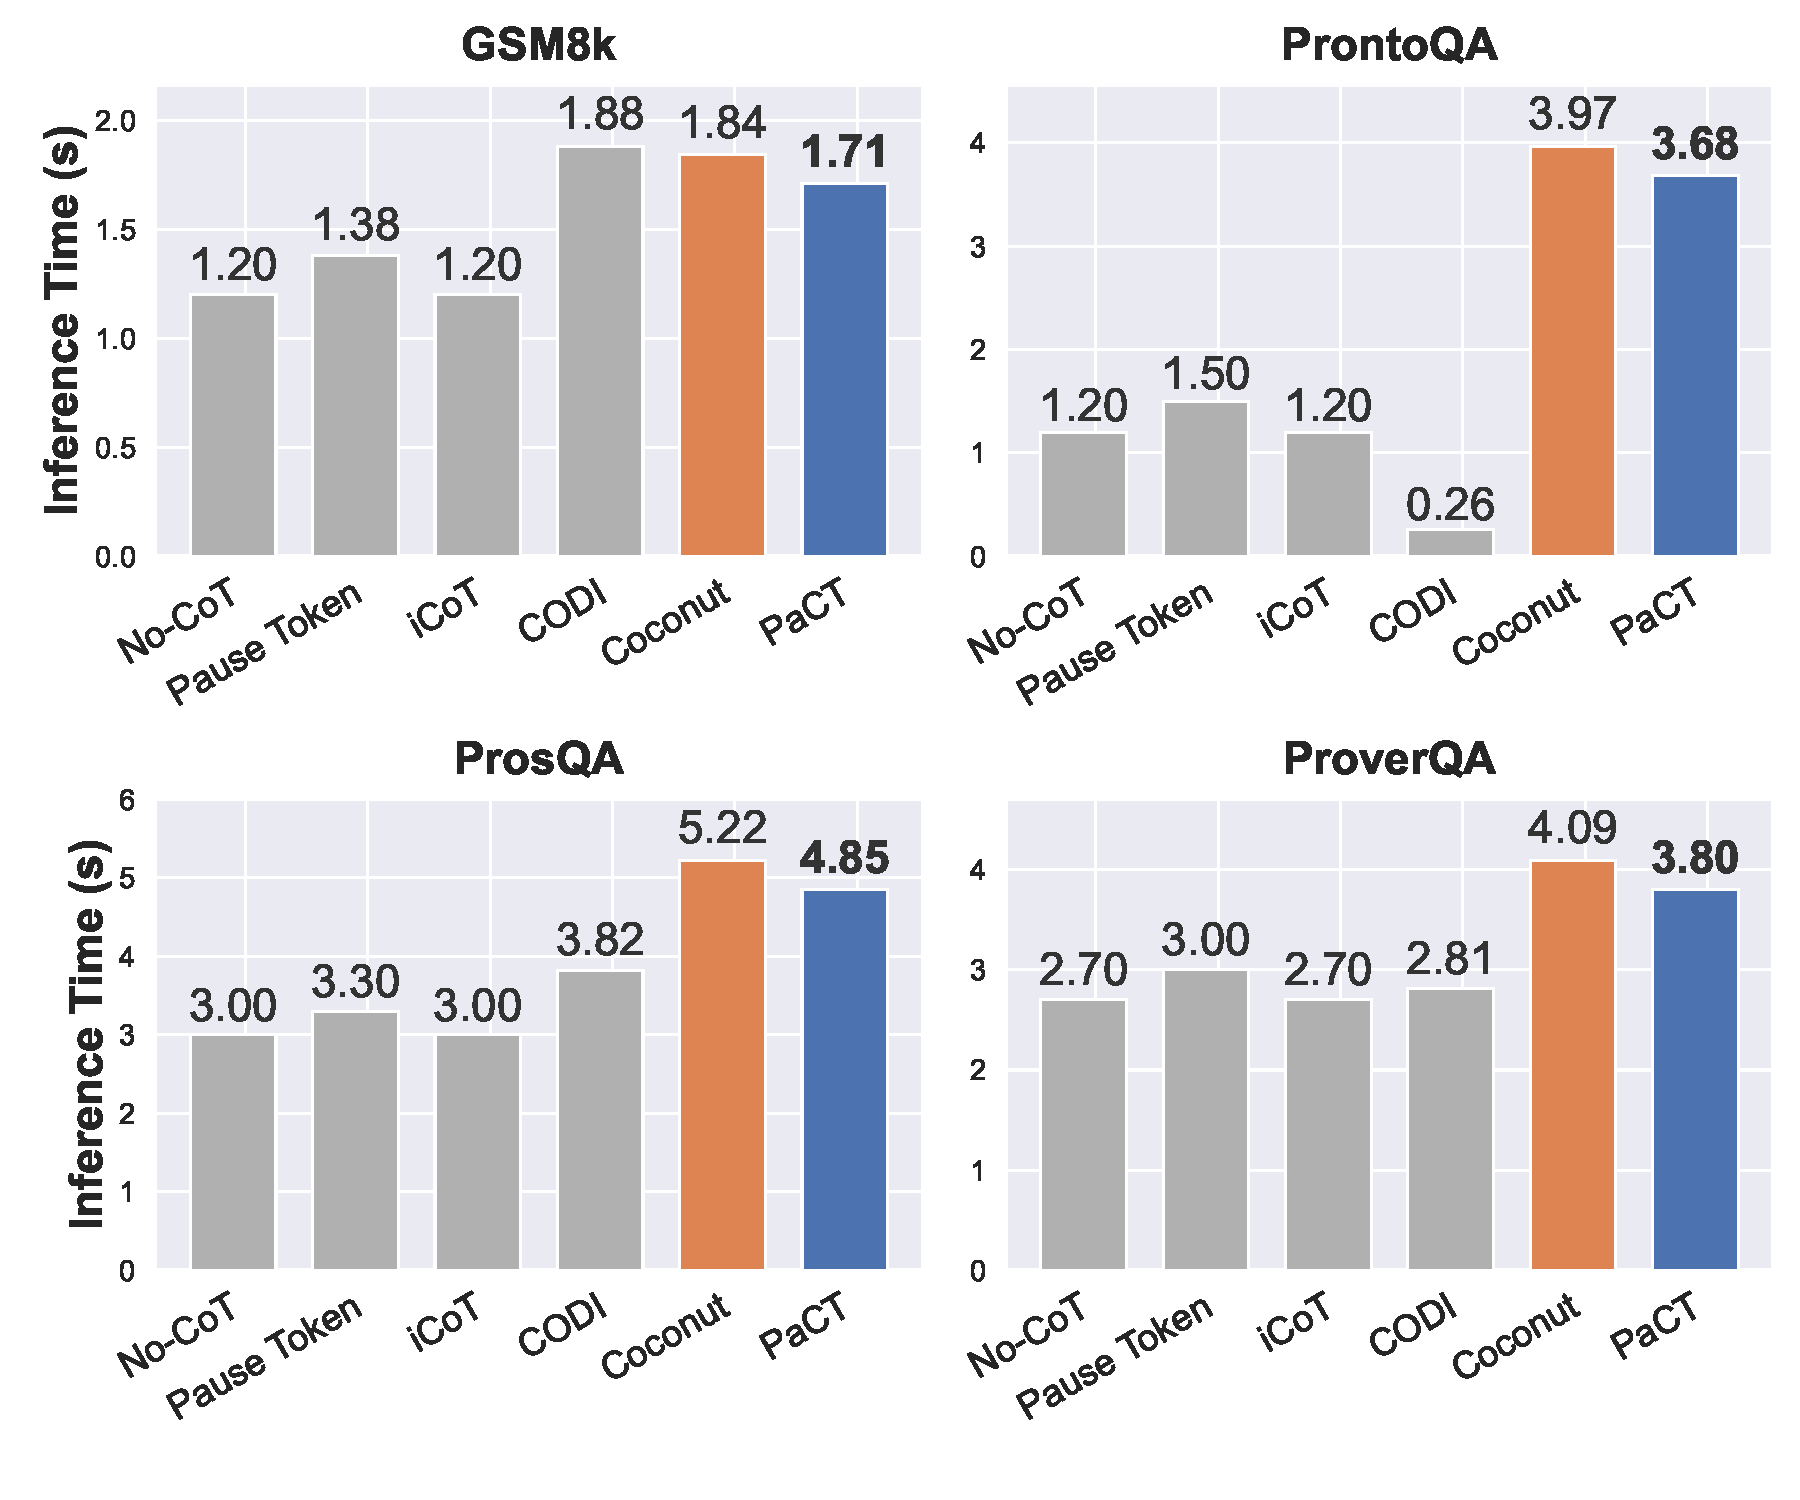
\includegraphics[width=\linewidth]{imgs/inference_times.pdf}
% %       \caption{Inference time (in seconds) for different reasoning methods across four benchmarks. PaCT demonstrates consistently lower latency compared to Coconut while maintaining competitive performance over baseline approaches.}
% %   \label{fig:inference_time}
% % \end{figure}
% %%%%%%%%%%%%%%%%%%%%%%%%%%%%%%%%%%%%%%%%%%%%%%%%%%%%%%%%%%%%%%%%%%%%%%%%%%%%%%%


% \section{Stability and initialization details}
% \label{app:stability}

% To stabilize optimization, we ground latent reasoning states in the task specification. Let $h_q$
% denote the hidden state of the final question token. We initialize the output projection of the latent
% synthesis cross-attention to zero and add $h_q$ as a residual to each latent state after synthesis.
% This ensures that, at initialization, all latent states correspond to grounded copies of the question
% representation and only deviate when learning discovers useful refinements.

% This grounding serves two purposes: (i) it anchors latent reasoning to the task context throughout
% training, and (ii) it prevents unstructured accumulation of latent history by ensuring that each
% stage depends only on the current textual context and a fixed task representation.

% \section{Attention masking and causal structure}
% \label{app:masking}

% We enforce the following attention constraints:
% \begin{enumerate}
%   \item Text tokens attend causally to earlier text tokens.
%   \item Text tokens do not attend to future latent states.
%   \item Latent states attend to all previous text tokens and to other latent states within the same
%   stage bidirectionally.
%   \item Answer tokens attend to all prior text tokens and all latent states from previous stages.
% \end{enumerate}
% This realizes a \emph{Text $\rightarrow$ Latents $\rightarrow$ Text} pattern while preserving
% autoregressive decoding and preventing label leakage.

% \section{Training algorithm}
% \label{app:algorithm}

% Algorithm~\ref{alg:pact_training} provides the full curriculum training procedure for PaCT.

% \begin{algorithm}[h]
% \caption{Curriculum training for PaCT}
% \label{alg:pact_training}
% \begin{algorithmic}[1]
% \Require Dataset $\mathcal{D}$, curriculum schedule $\{m_s,S_s\}$, slots $L$, parameters $\theta$, stepsize $\eta$
% \For{$s=0,\dots,S_{\max}$}
%   \For{$(q,r,a)\sim \mathcal{D}$}
%     \State Replace first $m_s$ rationale tokens in $r$ with $S_s$ latent stages
%     \State $x \leftarrow [\,q;\ \tilde{r}_s;\ a\,]$
%     \State Compute $p_\theta(\cdot\mid x)$ and latent states $Z'^{(1:S_s)}$
%     \State Update $\theta \leftarrow \theta - \eta \nabla_\theta \mathcal{L}(\theta)$
%   \EndFor
% \EndFor
% \end{algorithmic}
% \end{algorithm}


% \begin{figure}[h!]
%   \centering
%   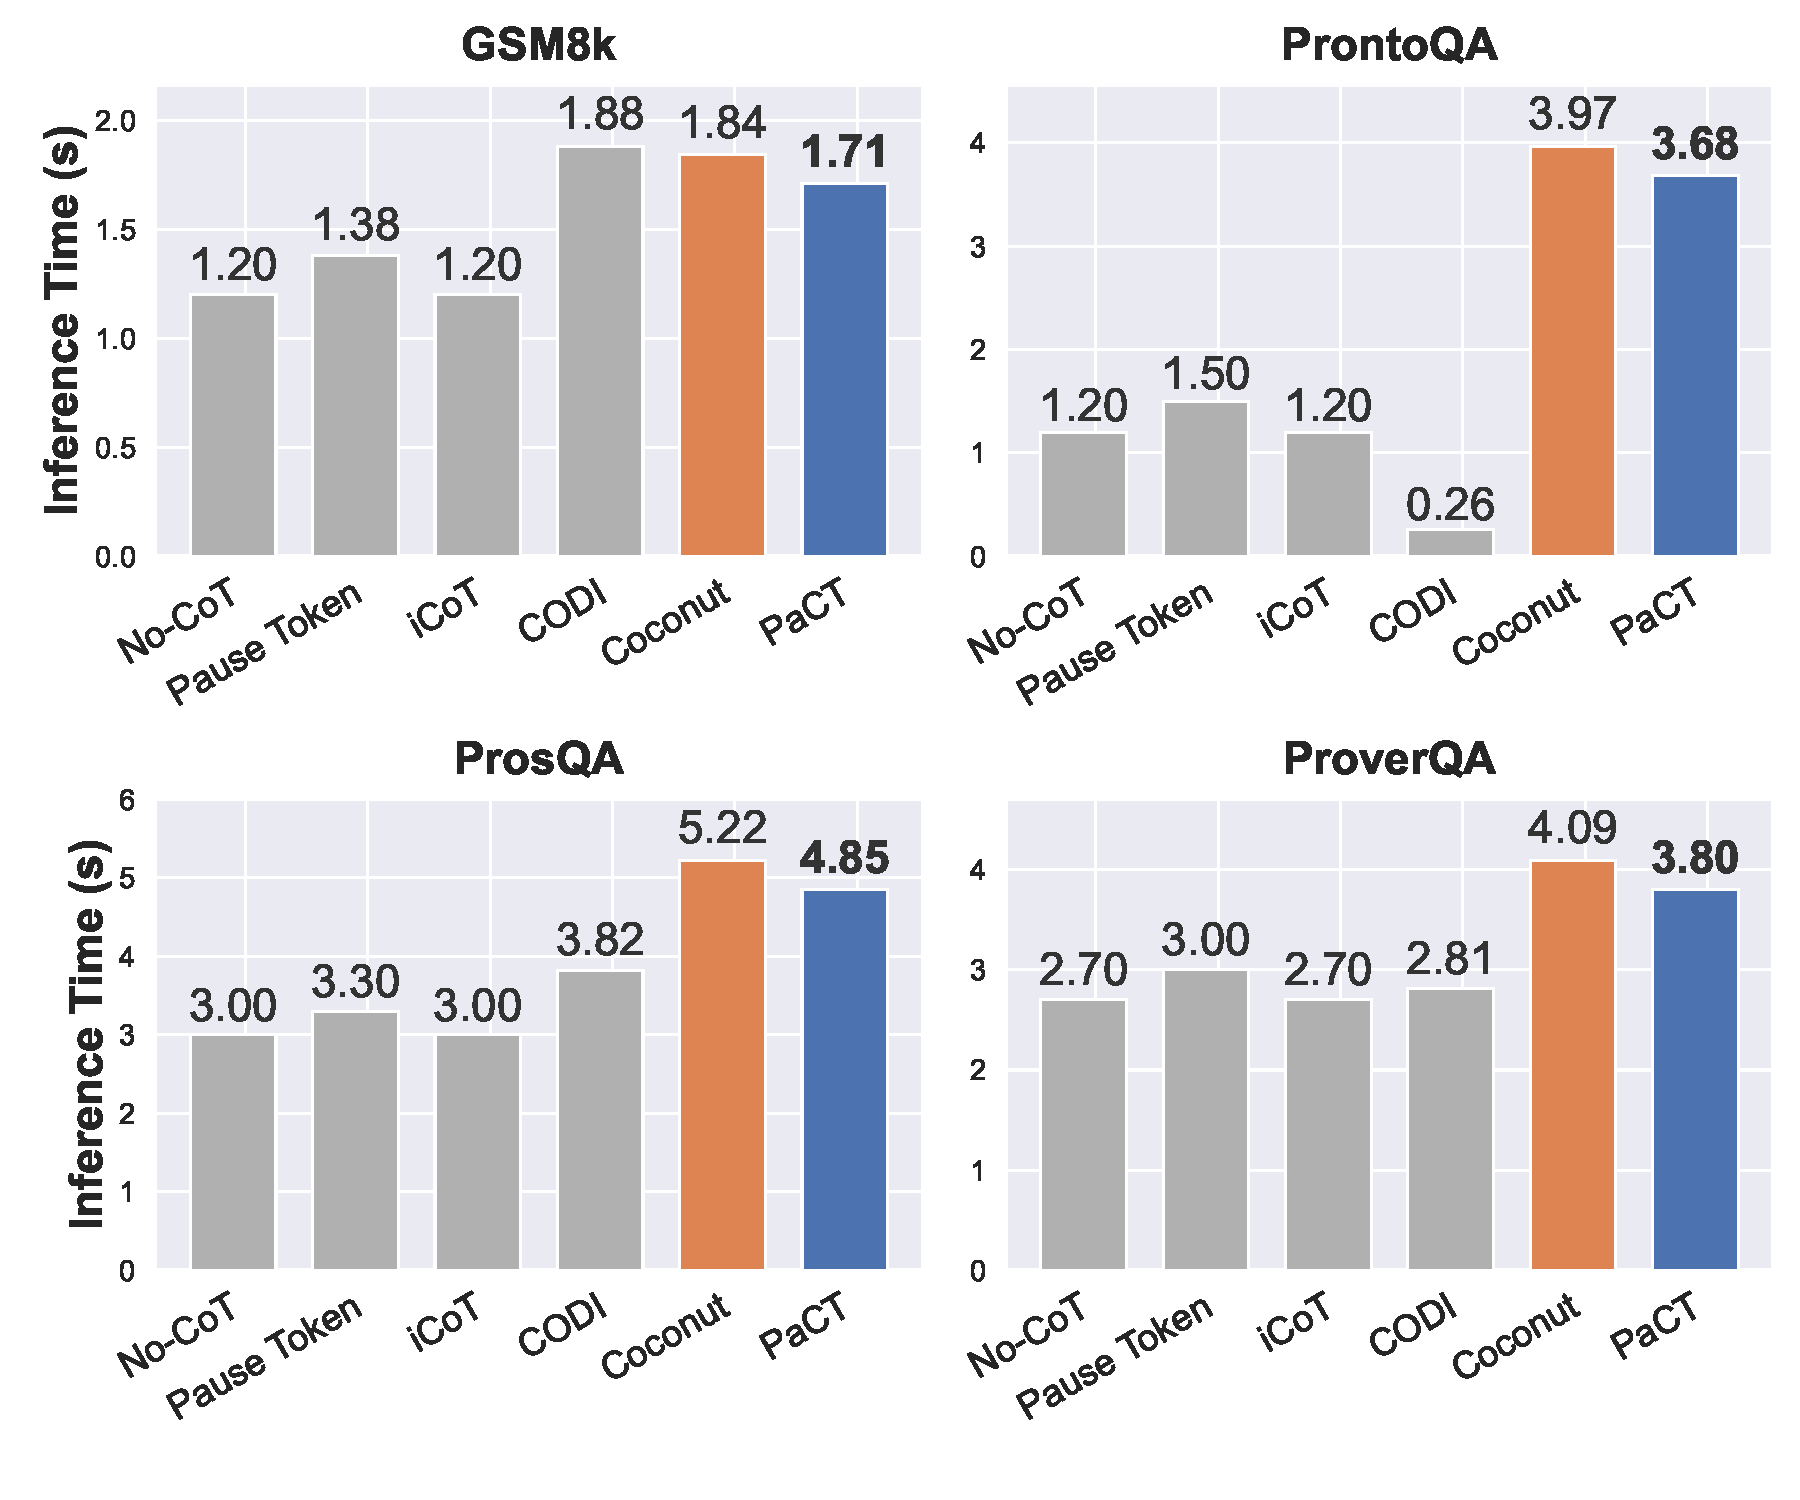
\includegraphics[width=\linewidth]{imgs/inference_times.pdf}
%       \caption{Inference time (in seconds) for different reasoning methods across four benchmarks. PaCT demonstrates consistently lower latency compared to Coconut while maintaining competitive performance over baseline approaches.}
%   \label{fig:inference_time}
% \end{figure}


% \begin{subfigure}[b]{0.48\textwidth}
%         \centering
%         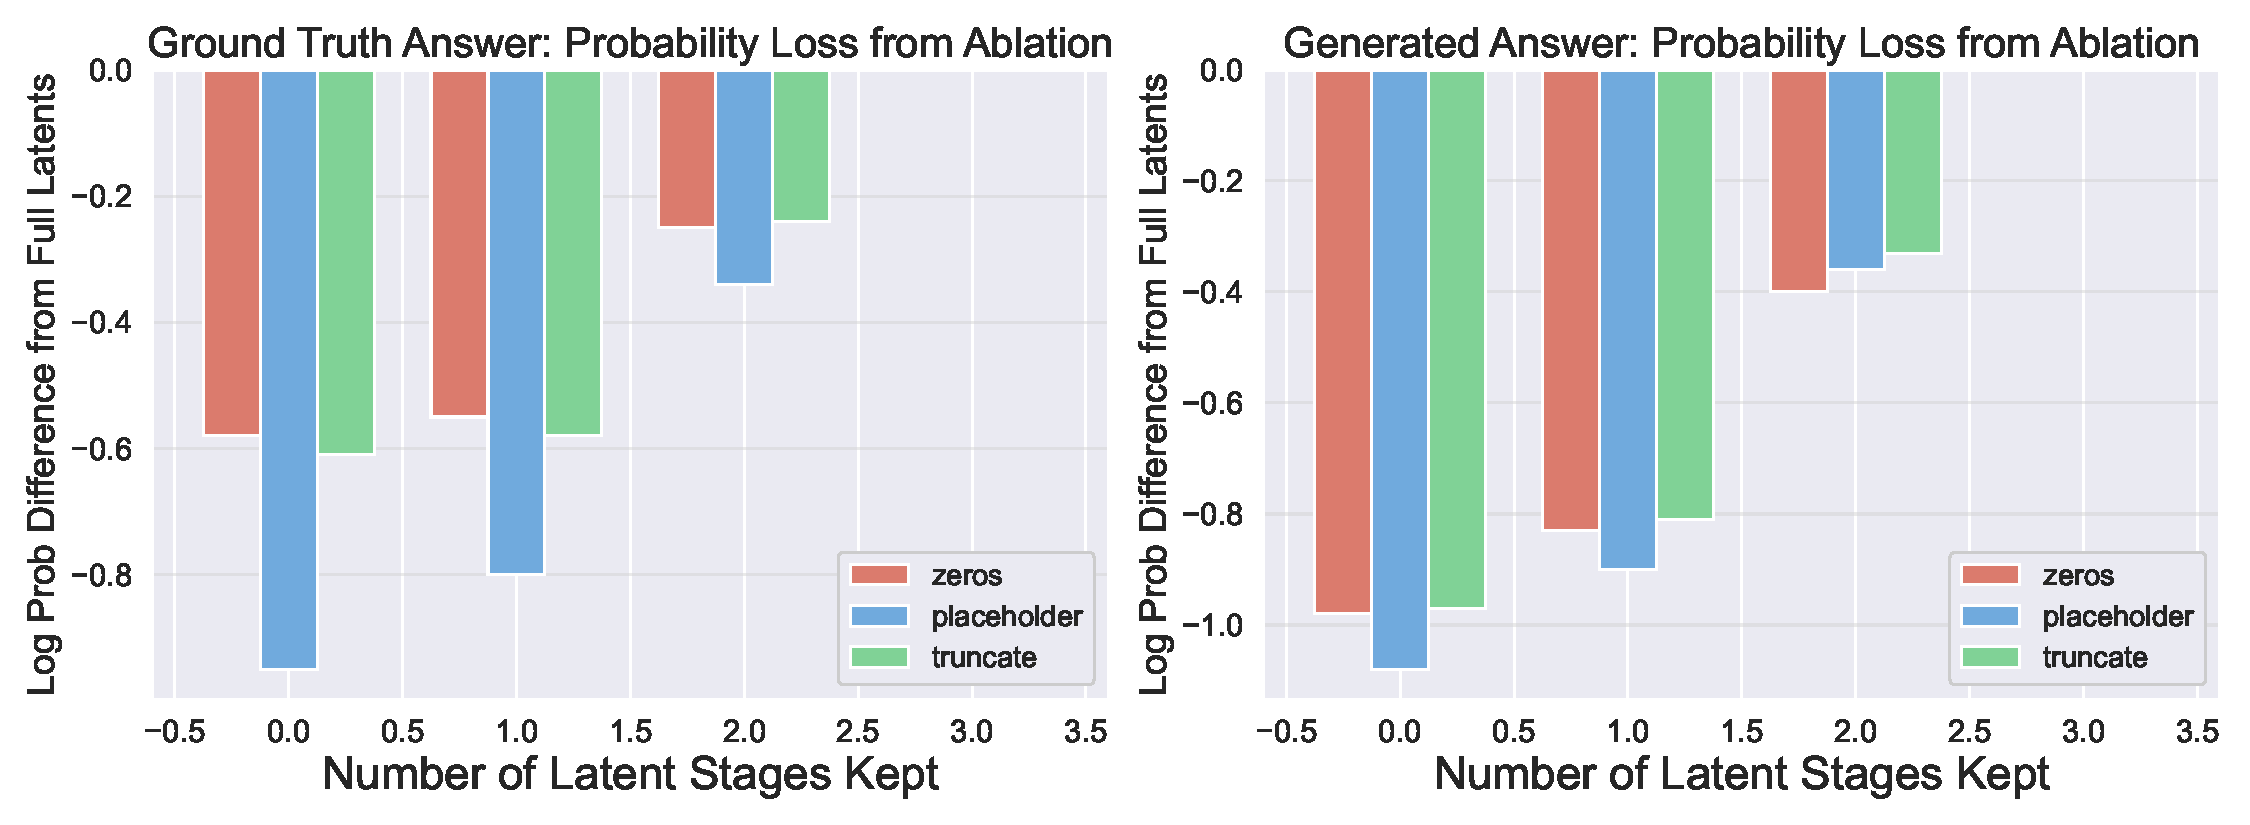
\includegraphics[width=\textwidth]{imgs/difference_from_baseline.pdf}
%         \caption{Difference from baseline}
%         \label{fig:ablation_diff}
%     \end{subfigure}


% \section{Additional Results and Ablations}
% \label{app:additional_results}

% \subsection{Log-probability drop relative to the full-latent baseline}
% \label{app:ablation_delta}

% \begin{figure}[t]
%   \centering
%   \includegraphics[width=\linewidth]{imgs/ablation_log_probs_delta.pdf}
%   \caption{\textbf{Stage ablation (relative view).} Log-probability drop relative to the full-latent baseline as a function of the number of stages retained. This view complements Fig.~\ref{fig:ablation_abs} by emphasizing the marginal value of additional stages. \textbf{[TODO: ensure the figure file name/path matches your repo; in the current PDF this plot appears as an additional figure-style panel.]}}
%   \label{fig:ablation_delta}
% \end{figure}

% \subsection{Depth sweep table for GSM8k}
% \label{app:depth_sweep_table}

% \begin{table}[t]
% \centering
% \small
% \caption{\textbf{Depth scaling on GSM8k (sweep).} Accuracy as a function of the number of stages on GSM8k with $c_{\text{thought}}=2$. \textbf{[TODO: clarify seeds/averaging for this sweep and reconcile the $S{=}3$ value with Table~\ref{tab:main_results} if they come from different runs.]}}
% \label{tab:stage_scaling}
% \begin{tabular}{l l c c}
% \toprule
% Method & Dataset & Accuracy (\%) & \# Stages \\
% \midrule
% Coconut & GSM8k & 34.2 & 3 \\
% PaCT    & GSM8k & 34.8 & 3 \\
% PaCT    & GSM8k & 36.6 & 6 \\
% PaCT    & GSM8k & 37.2 & 8 \\
% \bottomrule
% \end{tabular}
% \end{table}

% \subsection{Width and test-time truncation}
% \label{app:width_truncation}

% \begin{table}[t]
% \centering
% \small
% \caption{\textbf{Single-latent PaCT vs.\ dual-latent Coconut on GSM8k.} PaCT with $c_{\text{thought}}{=}1$ remains competitive with Coconut using $c_{\text{thought}}{=}2$, suggesting within-stage redundancy in PaCT.}
% \label{tab:1v2}
% \begin{tabular}{lcc}
% \toprule
% Model & $c_{\text{thought}}$ & Accuracy (\%) \\
% \midrule
% PaCT    & 1 & 33.20 \\
% Coconut & 2 & 32.00 \\
% \bottomrule
% \end{tabular}
% \end{table}

% \begin{table}[t]
% \centering
% \small
% \caption{\textbf{Test-time truncation of within-stage latents.} Accuracy when keeping only one of the two latent states per stage for a PaCT model trained with $c_{\text{thought}}=2$ and $S=3$ (GSM8k).}
% \label{tab:latent_redundancy}
% \begin{tabular}{lcc}
% \toprule
% Configuration & \# Latents & Accuracy (\%) \\
% \midrule
% Full model & 6 & 34.4 \\
% First of each stage (L0, L2, L4) & 3 & 31.6 \\
% Second of each stage (L1, L3, L5) & 3 & 31.6 \\
% \bottomrule
% \end{tabular}
% \end{table}

% \subsection{Effect of cross-attention context length}
% \label{app:context_length}

% \begin{table}[t]
%     \centering
%     \caption{\textbf{Effect of context length on GSM8k.} Accuracy for different numbers of context tokens (\texttt{num\_ctx}) used as keys/values in cross-attention.}
%     \label{tab:gpt2_gsm8k_context}
%     \begin{tabular}{lcc}
%         \toprule
%         Model & \texttt{num\_ctx} & Accuracy (\%) \\
%         \midrule
%         GPT-2 & 2   & 34.4 \\
%         GPT-2 & 4   & 33.0 \\
%         GPT-2 & 8   & 34.4 \\
%         GPT-2 & All & 30.6 \\
%         \bottomrule
%     \end{tabular}
% \end{table}

% \begin{figure}[t]
%   \centering
%   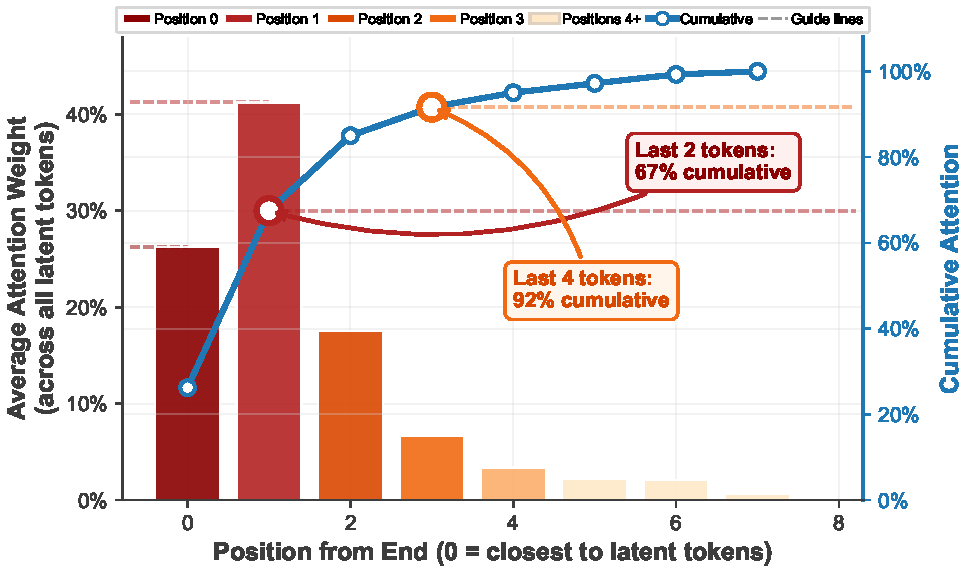
\includegraphics[width=\linewidth]{imgs/cross_attention_bias.pdf}
%   \caption{\textbf{Cross-attention concentrates on recent tokens.} Average attention weight as a function of position from the end of the prefix (0 = closest to the latent insertion point). Even with longer windows, attention mass concentrates on the last 1--2 hidden states, and cumulative attention saturates quickly.}
%   \label{fig:attention_heatmap}
% \end{figure}

% Table~\ref{tab:gpt2_gsm8k_context} shows that using the full prefix as cross-attention context degrades accuracy, while small windows remain strong. Figure~\ref{fig:attention_heatmap} explains this behavior: attention concentrates heavily on the most recent hidden states even when more context is available (e.g., $\sim$67\% mass on the last two tokens and $\sim$92\% on the last four). This supports the design choice of using a short window, which keeps latent synthesis lightweight without removing information the model actually uses.
% \textbf{[TODO: if you want a citation here, add one that supports ``recency dominance'' in autoregressive decoding; otherwise drop the sentence to avoid a weak citation.]}
% % =========================
% % Appendix: additional results
% % =========================

% \appendix

% \section{Additional Results and Ablations}
% \label{app:additional_results}

% \subsection{Log-probability drop relative to the full-latent baseline}
% \label{app:ablation_delta}

% \begin{figure}[t]
%   \centering
%   \includegraphics[width=\linewidth]{imgs/ablation_log_probs_delta.pdf}
%   \caption{\textbf{Stage ablation (relative view).} Log-probability drop relative to the full-latent baseline as a function of the number of stages retained. This view complements Fig.~\ref{fig:ablation_abs} by emphasizing the marginal value of additional stages. \textbf{[TODO: ensure the figure file name/path matches your repo; in the current PDF this plot appears as an additional figure-style panel.]}}
%   \label{fig:ablation_delta}
% \end{figure}

% \subsection{Depth sweep table for GSM8k}
% \label{app:depth_sweep_table}

% \begin{table}[t]
% \centering
% \small
% \caption{\textbf{Depth scaling on GSM8k (sweep).} Accuracy as a function of the number of stages on GSM8k with $c_{\text{thought}}=2$. \textbf{[TODO: clarify seeds/averaging for this sweep and reconcile the $S{=}3$ value with Table~\ref{tab:main_results} if they come from different runs.]}}
% \label{tab:stage_scaling}
% \begin{tabular}{l l c c}
% \toprule
% Method & Dataset & Accuracy (\%) & \# Stages \\
% \midrule
% Coconut & GSM8k & 34.2 & 3 \\
% PaCT    & GSM8k & 34.8 & 3 \\
% PaCT    & GSM8k & 36.6 & 6 \\
% PaCT    & GSM8k & 37.2 & 8 \\
% \bottomrule
% \end{tabular}
% \end{table}

% \subsection{Width and test-time truncation}
% \label{app:width_truncation}

% \begin{table}[t]
% \centering
% \small
% \caption{\textbf{Single-latent PaCT vs.\ dual-latent Coconut on GSM8k.} PaCT with $c_{\text{thought}}{=}1$ remains competitive with Coconut using $c_{\text{thought}}{=}2$, suggesting within-stage redundancy in PaCT.}
% \label{tab:1v2}
% \begin{tabular}{lcc}
% \toprule
% Model & $c_{\text{thought}}$ & Accuracy (\%) \\
% \midrule
% PaCT    & 1 & 33.20 \\
% Coconut & 2 & 32.00 \\
% \bottomrule
% \end{tabular}
% \end{table}

% \begin{table}[t]
% \centering
% \small
% \caption{\textbf{Test-time truncation of within-stage latents.} Accuracy when keeping only one of the two latent states per stage for a PaCT model trained with $c_{\text{thought}}=2$ and $S=3$ (GSM8k).}
% \label{tab:latent_redundancy}
% \begin{tabular}{lcc}
% \toprule
% Configuration & \# Latents & Accuracy (\%) \\
% \midrule
% Full model & 6 & 34.4 \\
% First of each stage (L0, L2, L4) & 3 & 31.6 \\
% Second of each stage (L1, L3, L5) & 3 & 31.6 \\
% \bottomrule
% \end{tabular}
% \end{table}

% \subsection{Effect of cross-attention context length}
% \label{app:context_length}

% \begin{table}[t]
%     \centering
%     \caption{\textbf{Effect of context length on GSM8k.} Accuracy for different numbers of context tokens (\texttt{num\_ctx}) used as keys/values in cross-attention.}
%     \label{tab:gpt2_gsm8k_context}
%     \begin{tabular}{lcc}
%         \toprule
%         Model & \texttt{num\_ctx} & Accuracy (\%) \\
%         \midrule
%         GPT-2 & 2   & 34.4 \\
%         GPT-2 & 4   & 33.0 \\
%         GPT-2 & 8   & 34.4 \\
%         GPT-2 & All & 30.6 \\
%         \bottomrule
%     \end{tabular}
% \end{table}

% \begin{figure}[t]
%   \centering
%   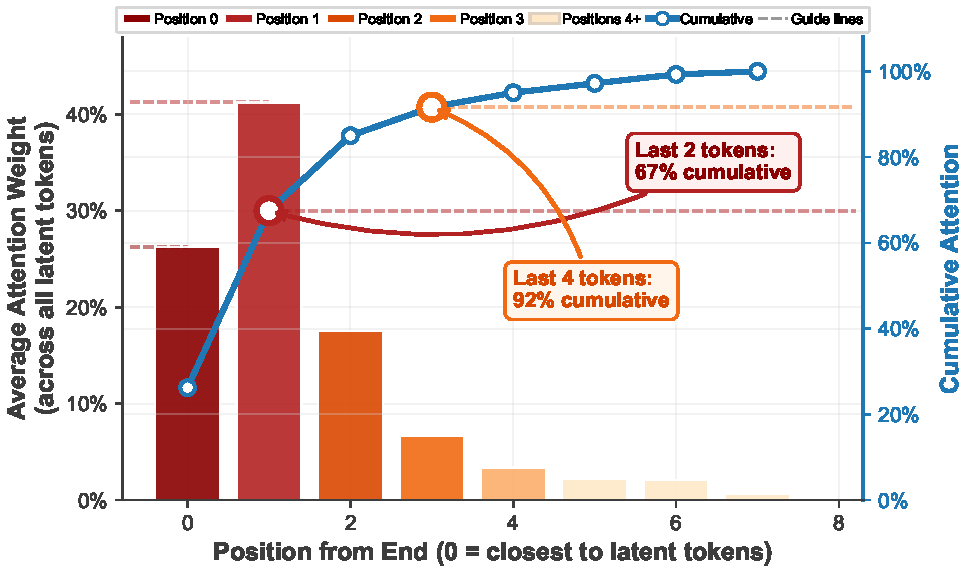
\includegraphics[width=\linewidth]{imgs/cross_attention_bias.pdf}
%   \caption{\textbf{Cross-attention concentrates on recent tokens.} Average attention weight as a function of position from the end of the prefix (0 = closest to the latent insertion point). Even with longer windows, attention mass concentrates on the last 1--2 hidden states, and cumulative attention saturates quickly.}
%   \label{fig:attention_heatmap}
% \end{figure}

% Table~\ref{tab:gpt2_gsm8k_context} shows that using the full prefix as cross-attention context degrades accuracy, while small windows remain strong. Figure~\ref{fig:attention_heatmap} explains this behavior: attention concentrates heavily on the most recent hidden states even when more context is available (e.g., $\sim$67\% mass on the last two tokens and $\sim$92\% on the last four). This supports the design choice of using a short window, which keeps latent synthesis lightweight without removing information the model actually uses.
% \textbf{[TODO: if you want a citation here, add one that supports ``recency dominance'' in autoregressive decoding; otherwise drop the sentence to avoid a weak citation.]}

% \subsection{Additional decoded latent examples}
% \label{app:more_examples}

% \begin{figure}[t]
% \centering
% \fbox{%
% \parbox{0.97\columnwidth}{
% \textbf{Example (Incorrect)} \hfill \textcolor{red}{\textbf{Incorrect}} \\[0.4em]
% \textbf{Question:} John cuts his grass to 2 inches. It grows 0.5 inches per month. When it gets to 4 inches he cuts it back down to 2 inches. It costs \$100 to get his grass cut. How much does he pay per year? \\[0.2em]
% \textbf{GT CoT:} $4{-}2=2 \rightarrow 2 \div 0.5 = 4$ months $\rightarrow 12 \div 4 = 3$ cuts $\rightarrow 100 \times 3 = 300$ \\[0.2em]
% \textbf{Predicted:} 200 \quad \textbf{GT:} 300 \\[0.4em]
% \begin{tabular}{c|cccccc}
% & L0 & L1 & L2 & L3 & L4 & L5 \\
% \hline
% Token & / & / & 200 & 200 & 200 & 5000 \\
% Prob  & 0.5\% & 0.4\% & 6.2\% & 11\% & 5.9\% & 8.5\% \\
% \end{tabular} \\[-0.2em]
% \textit{Interpretation:} Low and unstable confidence accompanies an incorrect reasoning trajectory; the final latent diverges.
% }}
% \caption{Additional decoded latent example supporting the qualitative trends discussed in Sec.~\ref{sec:latent_decoding}.}
% \label{fig:more_decoded_examples}
% \end{figure}

% \end{document}

\newpage
\appendix
\onecolumn


\section{Stability and initialization details}
\label{app:stability}

To stabilize optimization, we ground latent reasoning states in the task specification. Let $h_q$
denote the hidden state of the final question token. We initialize the output projection of the latent
synthesis cross-attention to zero and add $h_q$ as a residual to each latent state after synthesis.
This ensures that, at initialization, all latent states correspond to grounded copies of the question
representation and only deviate when learning discovers useful refinements.

This grounding serves two purposes: (i) it anchors latent reasoning to the task context throughout
training, and (ii) it prevents unstructured accumulation of latent history by ensuring that each
stage depends only on the current textual context and a fixed task representation.

\section{Attention masking and causal structure}
\label{app:masking}

We enforce the following attention constraints:
\begin{enumerate}
  \item Text tokens attend causally to earlier text tokens.
  \item Text tokens do not attend to future latent states.
  \item Latent states attend to all previous text tokens and to other latent states within the same
  stage bidirectionally.
  \item Answer tokens attend to all prior text tokens and all latent states from previous stages.
\end{enumerate}
This realizes a \emph{Text $\rightarrow$ Latents $\rightarrow$ Text} pattern while preserving
autoregressive decoding and preventing label leakage.

\section{PaCT training algorithm}
\label{app:algorithm}

Algorithm~\ref{alg:pact_training} provides the full curriculum training procedure for PaCT.

\begin{algorithm}[h]
\caption{Curriculum training for PaCT}
\label{alg:pact_training}
\begin{algorithmic}[1]
\Require Dataset $\mathcal{D}$, curriculum schedule $\{m_s,S_s\}$, slots $L$, parameters $\theta$, stepsize $\eta$
\For{$s=0,\dots,S_{\max}$}
  \For{$(q,r,a)\sim \mathcal{D}$}
    \State Replace first $m_s$ textual CoT tokens in $r$ with $S_s$ latent stages
    \State $x \leftarrow [\,q;\ \tilde{r}_s;\ a\,]$
    \State Compute $p_\theta(\cdot\mid x)$ and latent states $Z'^{(1:S_s)}$
    \State Update $\theta \leftarrow \theta - \eta \nabla_\theta \mathcal{L}(\theta)$
  \EndFor
\EndFor
\end{algorithmic}
\end{algorithm}

\section{Ablations on Latent Tokens}
\label{app:additional_results}

This section studies how PaCT utilizes latent tokens, with a focus on latent capacity and redundancy. In particular, we analyze (i) whether PaCT can outperform recurrent latent reasoning using fewer latent tokens, and (ii) whether multiple latent tokens within the same stage encode complementary or redundant information at inference time.

\subsection{Single-Latent PaCT vs.\ Dual-Latent Coconut}
\label{sec:single_double}
We first examine the minimum latent capacity required for effective continuous latent reasoning. Coconut relies on recurrent latent unrolling, where multiple latent tokens are generated sequentially and each latent must carry forward information from previous steps. In contrast, PaCT synthesizes latent tokens in parallel from the current context, without propagating latent states across steps.
\begin{table}[h]
    \centering
    \small
    \caption{Single-latent PaCT vs.\ dual-latent Coconut on GSM8k.}
    \label{tab:1v2}
    \begin{tabular}{lcc}
        \toprule
        Model & $c_{\text{thought}}$ & Accuracy (\%) \\
        \midrule
        PaCT    & 1 & 33.20 \\
        Coconut & 2 & 32.00 \\
        \bottomrule
    \end{tabular}
\end{table}
To isolate the effect of latent capacity, we compare PaCT using a single latent token per stage ($c_{\text{thought}}=1$) against Coconut using two recurrently unrolled latent tokens ($c_{\text{thought}}=2$), following standard Coconut settings on GSM8k. As shown in Table~\ref{tab:1v2}, PaCT with only one latent token already outperforms Coconut (33.20\% vs.\ 32.00\%).

This result indicates that PaCT does not rely on increased latent width to achieve strong performance. Instead, its stage-wise, context-grounded latent resynthesis produces more information-dense latent representations, allowing PaCT to match or exceed the performance of recurrent latent reasoning while using fewer latent tokens.

\subsection{Latent Redundancy Within Stages}
\label{subsec:latent_redundancy}
We investigate whether multiple latent tokens within the same PaCT stage encode complementary information or exhibit redundancy. We consider a PaCT model trained with two latent tokens per stage and three stages ($c_{\text{thought}}=2$, $S=3$), resulting in six latent tokens in total. At inference time, we selectively retain only one latent token per stage, discarding the other.
\begin{table}[h]
    \centering
    \small
    \caption{Accuracy when keeping only 1 of 2 latents per stage (PaCT trained with $c_{\text{thought}}=2$, $S=3$ on GSM8k).}
    \label{tab:latent_redundancy}
    \begin{tabular}{lcc}
        \toprule
        Configuration & \# Latents & Accuracy (\%) \\
        \midrule
        Full model & 6 & 34.4 \\
        First of each stage (L0, L2, L4) & 3 & 31.6 \\
        Second of each stage (L1, L3, L5) & 3 & 31.6 \\
        \bottomrule
    \end{tabular}
\end{table}

Table~\ref{tab:latent_redundancy} reports the resulting accuracy. Retaining either the first or the second latent token from each stage yields identical performance (31.6\%), regardless of which latent is kept. Although accuracy decreases relative to the full model (34.4\%), the symmetry across configurations indicates that latent tokens within the same stage encode largely redundant information.

This observation is consistent with the high within-stage similarity measured in our latent similarity analysis and supports the design choice of allocating compute toward greater depth (more stages) rather than increased latent width. In PaCT, reasoning benefits more from additional stages than from duplicating latent capacity within a stage.


\section{Latent decoding analysis -- extension}
\label{app:latent_decoding_examples}

This section provides additional qualitative evidence to complement the latent decoding analysis in Sec.~\ref{sec:latent_decoding}. Our goal is not to claim that latent reasoning states correspond to explicit natural language tokens, but rather to probe whether latent trajectories encode meaningful intermediate computations that align with the ground-truth reasoning process.

\begin{algorithm}[h ]
\caption{Top-$k$ Latent Decoding Probe for PaCT/Coconut ($k{=}5$)}
\label{alg:latent_probe_topk}
\begin{algorithmic}[1]
\Require Transformer $f_{\theta}$ with latent stages, output matrix $W_{\text{out}} \in \mathbb{R}^{|\mathcal{V}|\times d}$, input $x$, stages $S$
\Ensure Top-$k$ trajectories $\{(V_s, P_s)\}_{s=1}^{S}$
\State Compute latent embeddings $\{z_s \in \mathbb{R}^d\}_{s=1}^{S} \leftarrow f_{\theta}(x)$
\For{$s = 1, \ldots, S$}
    \State $\ell_s \leftarrow W_{\text{out}} z_s$
    \State $p_s \leftarrow \text{softmax}(\ell_s)$
    \State $V_s \leftarrow \text{top-}k(p_s)$, $P_s \leftarrow \{p_s(v) \mid v \in V_s\}$
\EndFor
\State \textbf{return} $\{(V_s, P_s)\}_{s=1}^{S}$
\end{algorithmic}
\end{algorithm}

We provide additional decoded latent trajectories to supplement Sec.~\ref{sec:latent_decoding}.


\paragraph{Top-$k$ latent decoding probe.}
We apply the Top-$k$ Latent Decoding Probe (Alg.~\ref{alg:latent_probe_topk}) to both PaCT and Coconut models. For each latent state, we project the latent embedding into vocabulary space using the output projection matrix and inspect the top-$k$ tokens along with their probabilities. This probe serves as a diagnostic tool to visualize how internal latent representations evolve across reasoning stages and whether they track intermediate quantities relevant to the final answer.

\paragraph{Progressive refinement in PaCT.}
Across correct examples (Examples S1--S2), PaCT exhibits a clear stage-wise progression from intermediate quantities toward the final answer. Early latent stages often decode to coarse intermediate values (e.g., partial sums or products), while later stages increasingly concentrate probability mass on the correct final answer. Importantly, latent pairs within the same stage frequently decode to identical tokens with similar probabilities, reflecting the high within-stage similarity reported in Table~4 of the main paper. This behavior is consistent with PaCT's design: latent states within a stage act as parallel hypotheses derived from the same contextual grounding, rather than representing sequential reasoning steps.

\vspace{0.8em}
\noindent\fbox{\parbox{0.97\textwidth}{
\textbf{Example S1} \hfill \textcolor{green!60!black}{\textbf{Correct}} \\[0.4em]
\textbf{Question:} Maggie went to Lou's aquarium and saw 100 goldfish. She was allowed to catch half, and she caught $3/5$ of that. How many remain to catch? \\[0.2em]
\textbf{Ground Truth CoT:} $100 \times \frac{1}{2} = 50 \rightarrow 50 \times \frac{3}{5} = 30 \rightarrow 50 - 30 = 20$ \\[0.2em]
\textbf{Predicted:} 20 \quad \textbf{GT:} 20 \\[0.4em]
\begin{tabular}{c|cccccc}
& L0 & L1 & L2 & L3 & L4 & L5 \\
\hline
Token & \textbf{50} & \textbf{50} & \textbf{30} & \textbf{30} & \textbf{20} & \textbf{20} \\
Prob  & 13\% & 14\% & 13\% & 20\% & 55\% & 56\% \\
\end{tabular} \\[-0.2em]
\textit{Interpretation:} Intermediate-to-final progression with sharpening confidence.
}}

\vspace{0.8em}
\noindent\fbox{\parbox{0.97\textwidth}{
\textbf{Example S2} \hfill \textcolor{green!60!black}{\textbf{Correct}} \\[0.4em]
\textbf{Question:} Mitchell has 8 packets of gum, 7 pieces each, and chews all but 2. How many does he chew? \\[0.2em]
\textbf{Ground Truth CoT:} $8 \times 7 = 56 \rightarrow 56 - 2 = 54$ \\[0.2em]
\textbf{Predicted:} 54 \quad \textbf{GT:} 54 \\[0.4em]
\begin{tabular}{c|cccccc}
& L0 & L1 & L2 & L3 & L4 & L5 \\
\hline
Token & \textbf{56} & \textbf{56} & \textbf{54} & \textbf{54} & \textbf{54} & \textbf{54} \\
Prob  & 5.2\% & 6.5\% & 25\% & 50\% & 87\% & 83\% \\
\end{tabular} \\[-0.2em]
\textit{Interpretation:} Answer emerges early and confidence sharpens across stages.
}}

\vspace{0.8em}
\noindent\fbox{\parbox{0.97\textwidth}{
\textbf{Example S3} \hfill \textcolor{red}{\textbf{Incorrect}} \\[0.4em]
\textbf{Question:} Roman and Remy used 33 gallons. Remy used $1$ more than $3\times$ Roman. How many did Remy use? \\[0.2em]
\textbf{Ground Truth CoT:} $x + (3x+1)=33 \rightarrow x=8 \rightarrow 3x+1=25$ \\[0.2em]
\textbf{Predicted:} 26.25 \quad \textbf{GT:} 25 \\[0.4em]
\begin{tabular}{c|cccccc}
& L0 & L1 & L2 & L3 & L4 & L5 \\
\hline
Token & 34 & 34 & 9 & 9 & \textbf{25} & \textbf{25} \\
Prob  & 11\% & 12\% & 7.5\% & 8.6\% & 22\% & 26\% \\
\end{tabular} \\[-0.2em]
\textit{Interpretation:} Latents reach the correct answer late, but decoding still commits to an incorrect output.
}}

\vspace{0.8em}
\noindent\fbox{\parbox{0.97\textwidth}{
\textbf{Example S4} \hfill \textcolor{red}{\textbf{Incorrect}} \\[0.4em]
\textbf{Question:} Suzy starts with 98 books. 43 checked out. Next day 23 returned and 5 checked out. Friday 7 returned. How many books? \\[0.2em]
\textbf{Ground Truth CoT:} $98-43=55 \rightarrow 55+23=78 \rightarrow 78-5=73 \rightarrow 73+7=80$ \\[0.2em]
\textbf{Predicted:} 119 \quad \textbf{GT:} 80 \\[0.4em]
\begin{tabular}{c|cccccc}
& L0 & L1 & L2 & L3 & L4 & L5 \\
\hline
Token & 69 & 69 & 76 & 72 & 70 & 70 \\
Prob  & 3.6\% & 3.4\% & 0.9\% & 1.6\% & 11\% & 9.3\% \\
\end{tabular} \\[-0.2em]
\textit{Interpretation:} Multi-step tracking fails; low probabilities reflect uncertainty.
}}

\vspace{0.8em}
\noindent\fbox{\parbox{0.97\textwidth}{
\textbf{Example S5} \hfill \textcolor{red}{\textbf{Incorrect}} \\[0.4em]
\textbf{Question:} Opera tickets increased from \$85 to \$102. What is the percent increase? \\[0.2em]
\textbf{Ground Truth CoT:} $102-85=17 \rightarrow \frac{17}{85}\times 100 = 20\%$ \\[0.2em]
\textbf{Predicted:} 12 \quad \textbf{GT:} 20 \\[0.4em]
\begin{tabular}{c|cccccc}
& L0 & L1 & L2 & L3 & L4 & L5 \\
\hline
Token & 73 & 73 & . & . & 12 & 12 \\
Prob  & 3.5\% & 3.1\% & 12\% & 18\% & 25\% & 24\% \\
\end{tabular} \\[-0.2em]
\textit{Interpretation:} Reasoning collapses; the model commits to an incorrect answer without computing the correct percentage.
}}

\paragraph{Failure modes and uncertainty signals.}
In incorrect cases (Examples S3--S5), the latent decoding probe reveals informative failure patterns. In some instances, PaCT latents reach the correct intermediate or even final value at later stages but fail to sustain sufficient confidence for correct decoding (Example S3). In others, the latent trajectory captures partial intermediates but fails to correctly compose them (Example S4), or collapses early to an incorrect estimate without completing the required computation (Example S5). These cases are characterized by low or diffuse probability mass across decoded tokens, indicating uncertainty rather than confident hallucination.

\paragraph{Comparison with Coconut.}
In contrast to PaCT, Coconut’s recurrently unrolled latent states exhibit less structured progression. Decoded tokens often fluctuate across stages, mix intermediate and irrelevant quantities, or prematurely terminate with end-of-text or non-numeric tokens. This behavior is consistent with Coconut’s recurrent latent propagation, where each latent must simultaneously carry forward prior information and perform new computation, leading to entangled representations and higher cross-stage similarity. As a result, Coconut latent trajectories are less interpretable and less aligned with the underlying arithmetic structure of the task.

Together, these extended examples reinforce three key observations. First, PaCT latent states encode meaningful intermediate quantities despite never being supervised to produce text. Second, reasoning in PaCT emerges as a stage-wise refinement process rather than a single evolving latent trajectory. Third, decoding probabilities provide a useful confidence signal: correct predictions are associated with sharpening probability mass on the final answer, while failures exhibit diffuse or unstable latent confidence. These findings support the claim that PaCT’s parallel, stage-wise latent resynthesis yields more structured and interpretable internal reasoning dynamics than recurrent latent unrolling.




\begin{figure}[t]
  \centering
  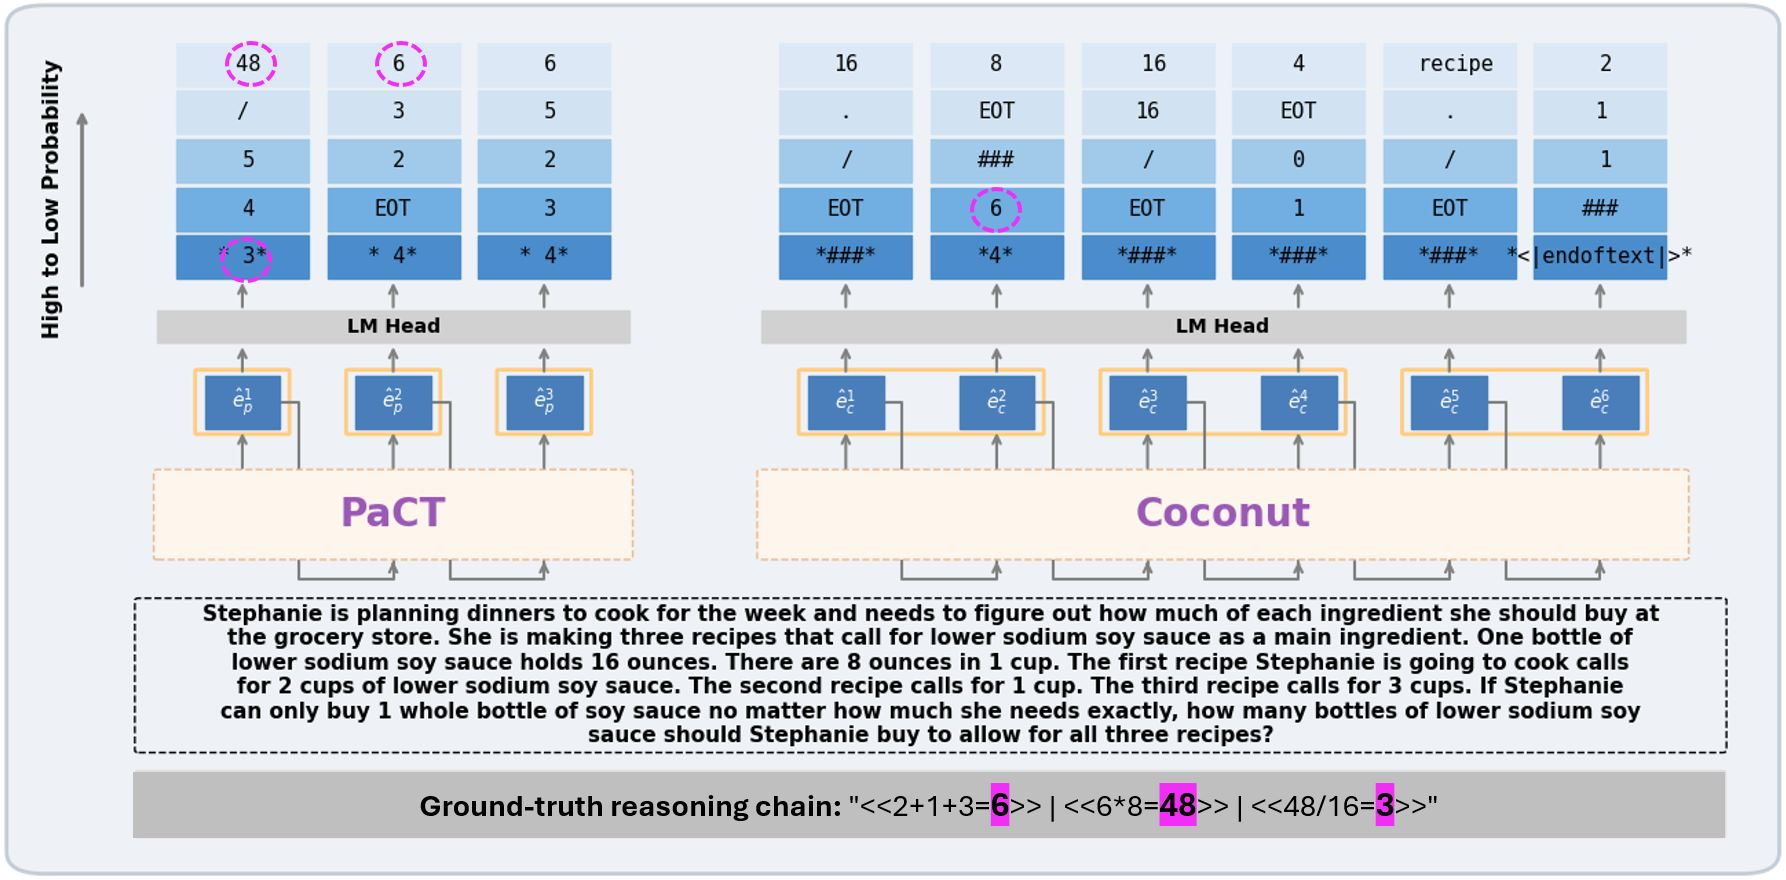
\includegraphics[width=\linewidth]{imgs/teaser2.JPG}
  \caption{\textbf{PaCT vs Coconut latent decoding comparison - example 1}}
  \label{fig:accuracy_and_latent_stages2}
\end{figure}

\begin{figure}[t]
  \centering
  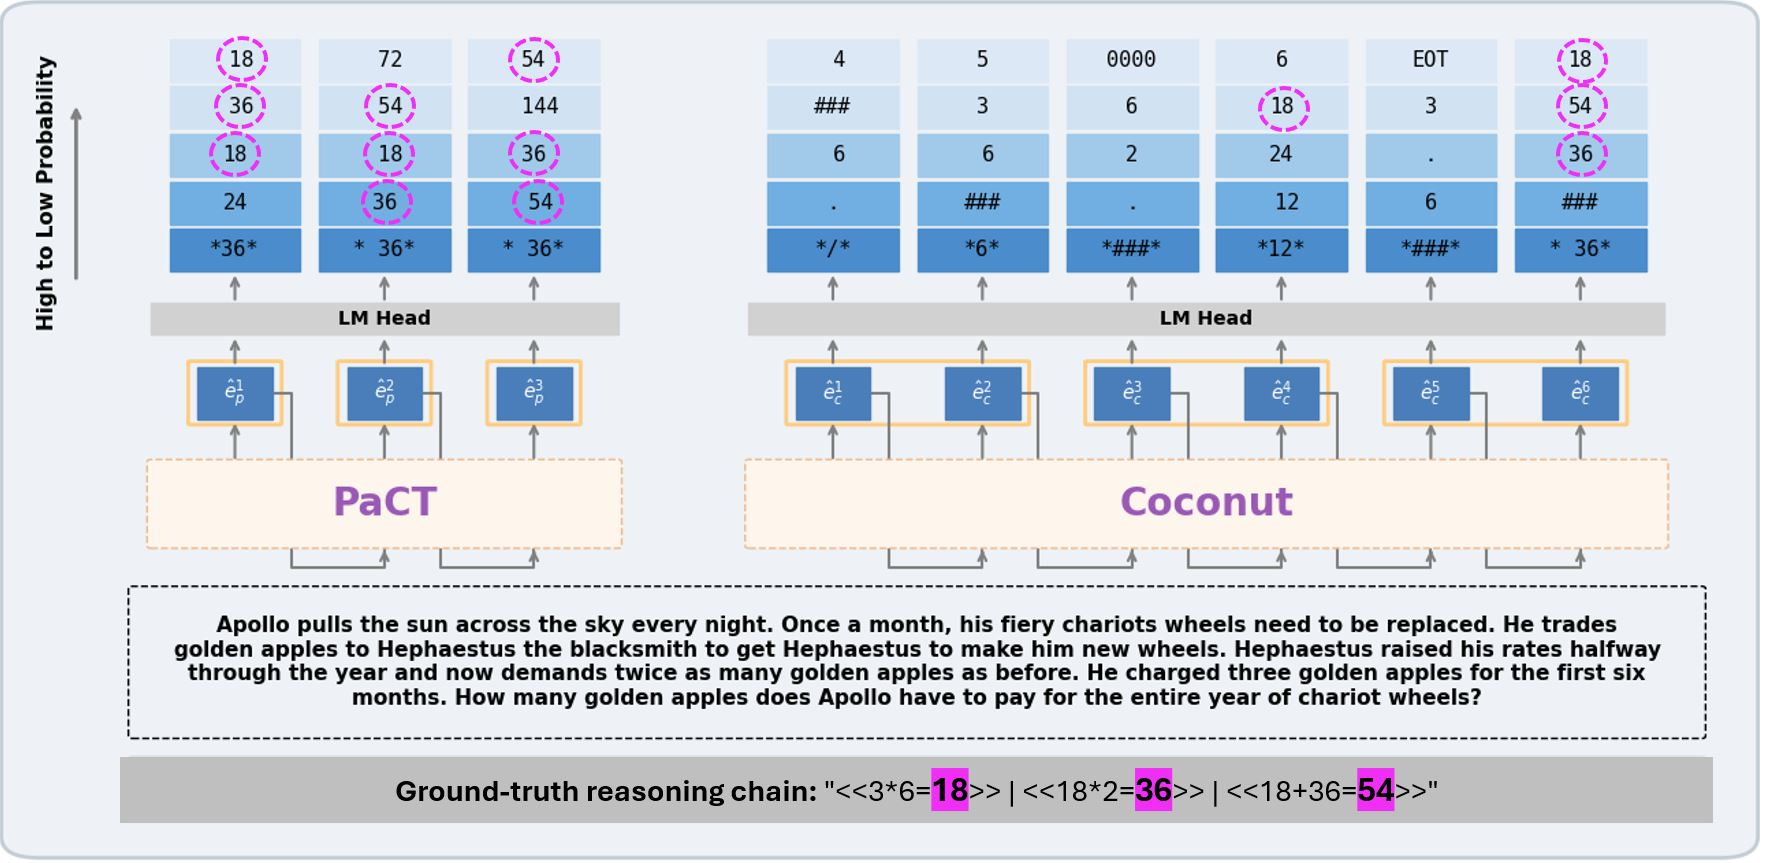
\includegraphics[width=\linewidth]{imgs/teaser3.JPG}
  \caption{\textbf{PaCT vs Coconut latent decoding comparison - example 2}}
  \label{fig:accuracy_and_latent_stages3}
\end{figure}

\begin{figure}[t]
  \centering
  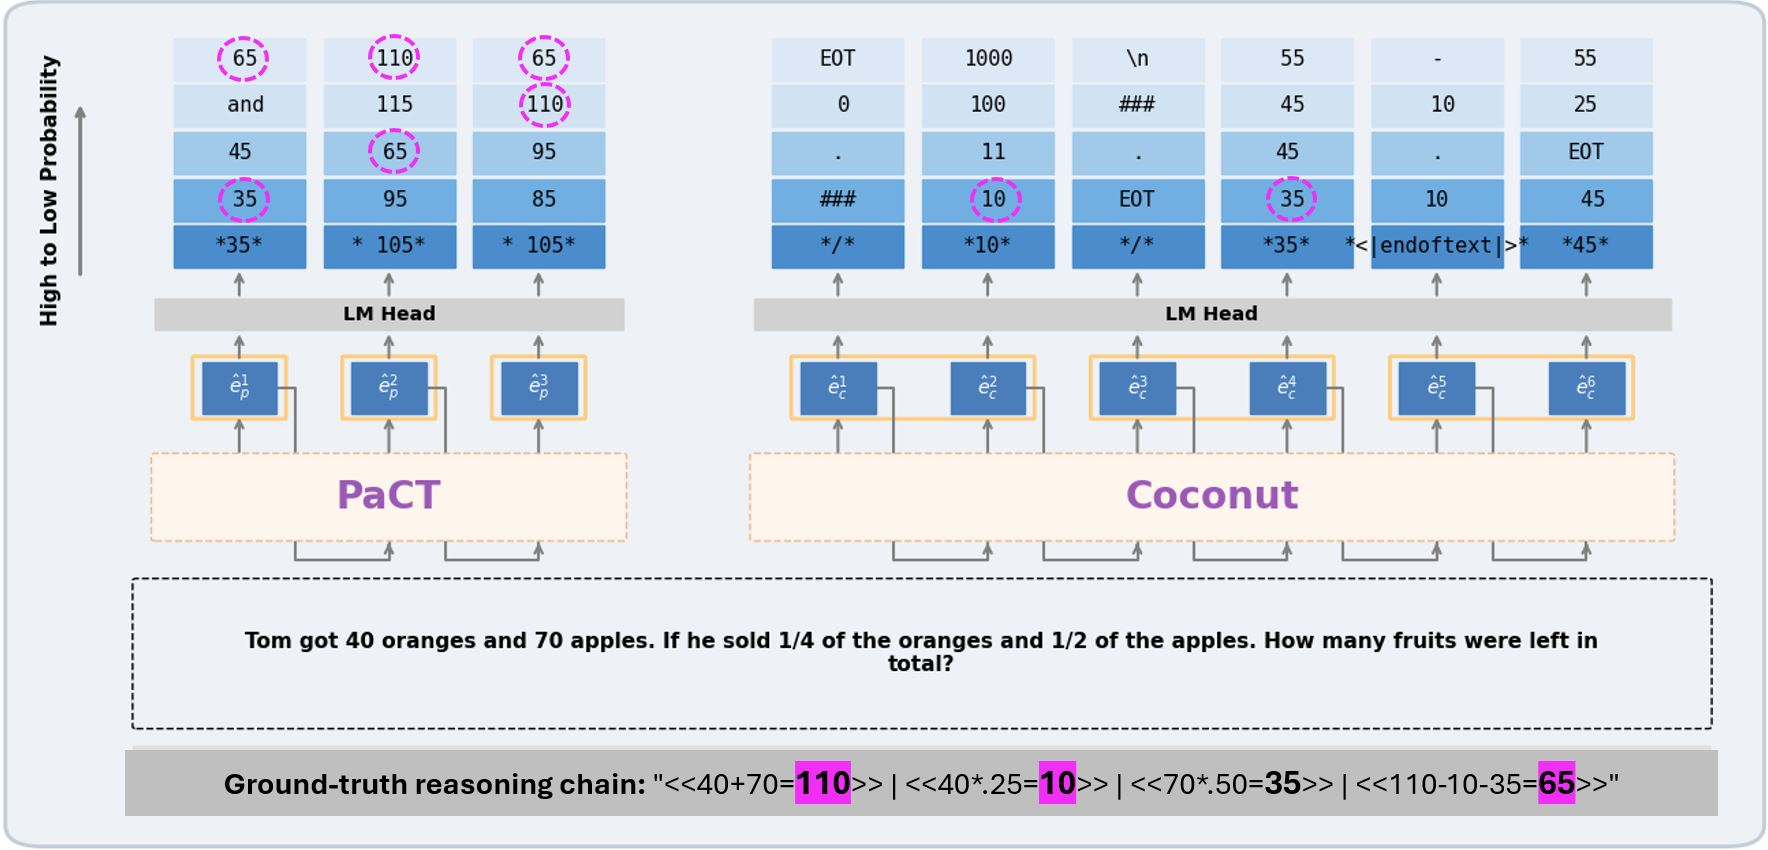
\includegraphics[width=\linewidth]{imgs/teaser4.JPG}
  \caption{\textbf{PaCT vs Coconut latent decoding comparison - example 3}}
  \label{fig:accuracy_and_latent_stages4}
\end{figure}



\section{Inference latency}
\label{sec:inference_latency}

\begin{figure}[t]
  \centering
  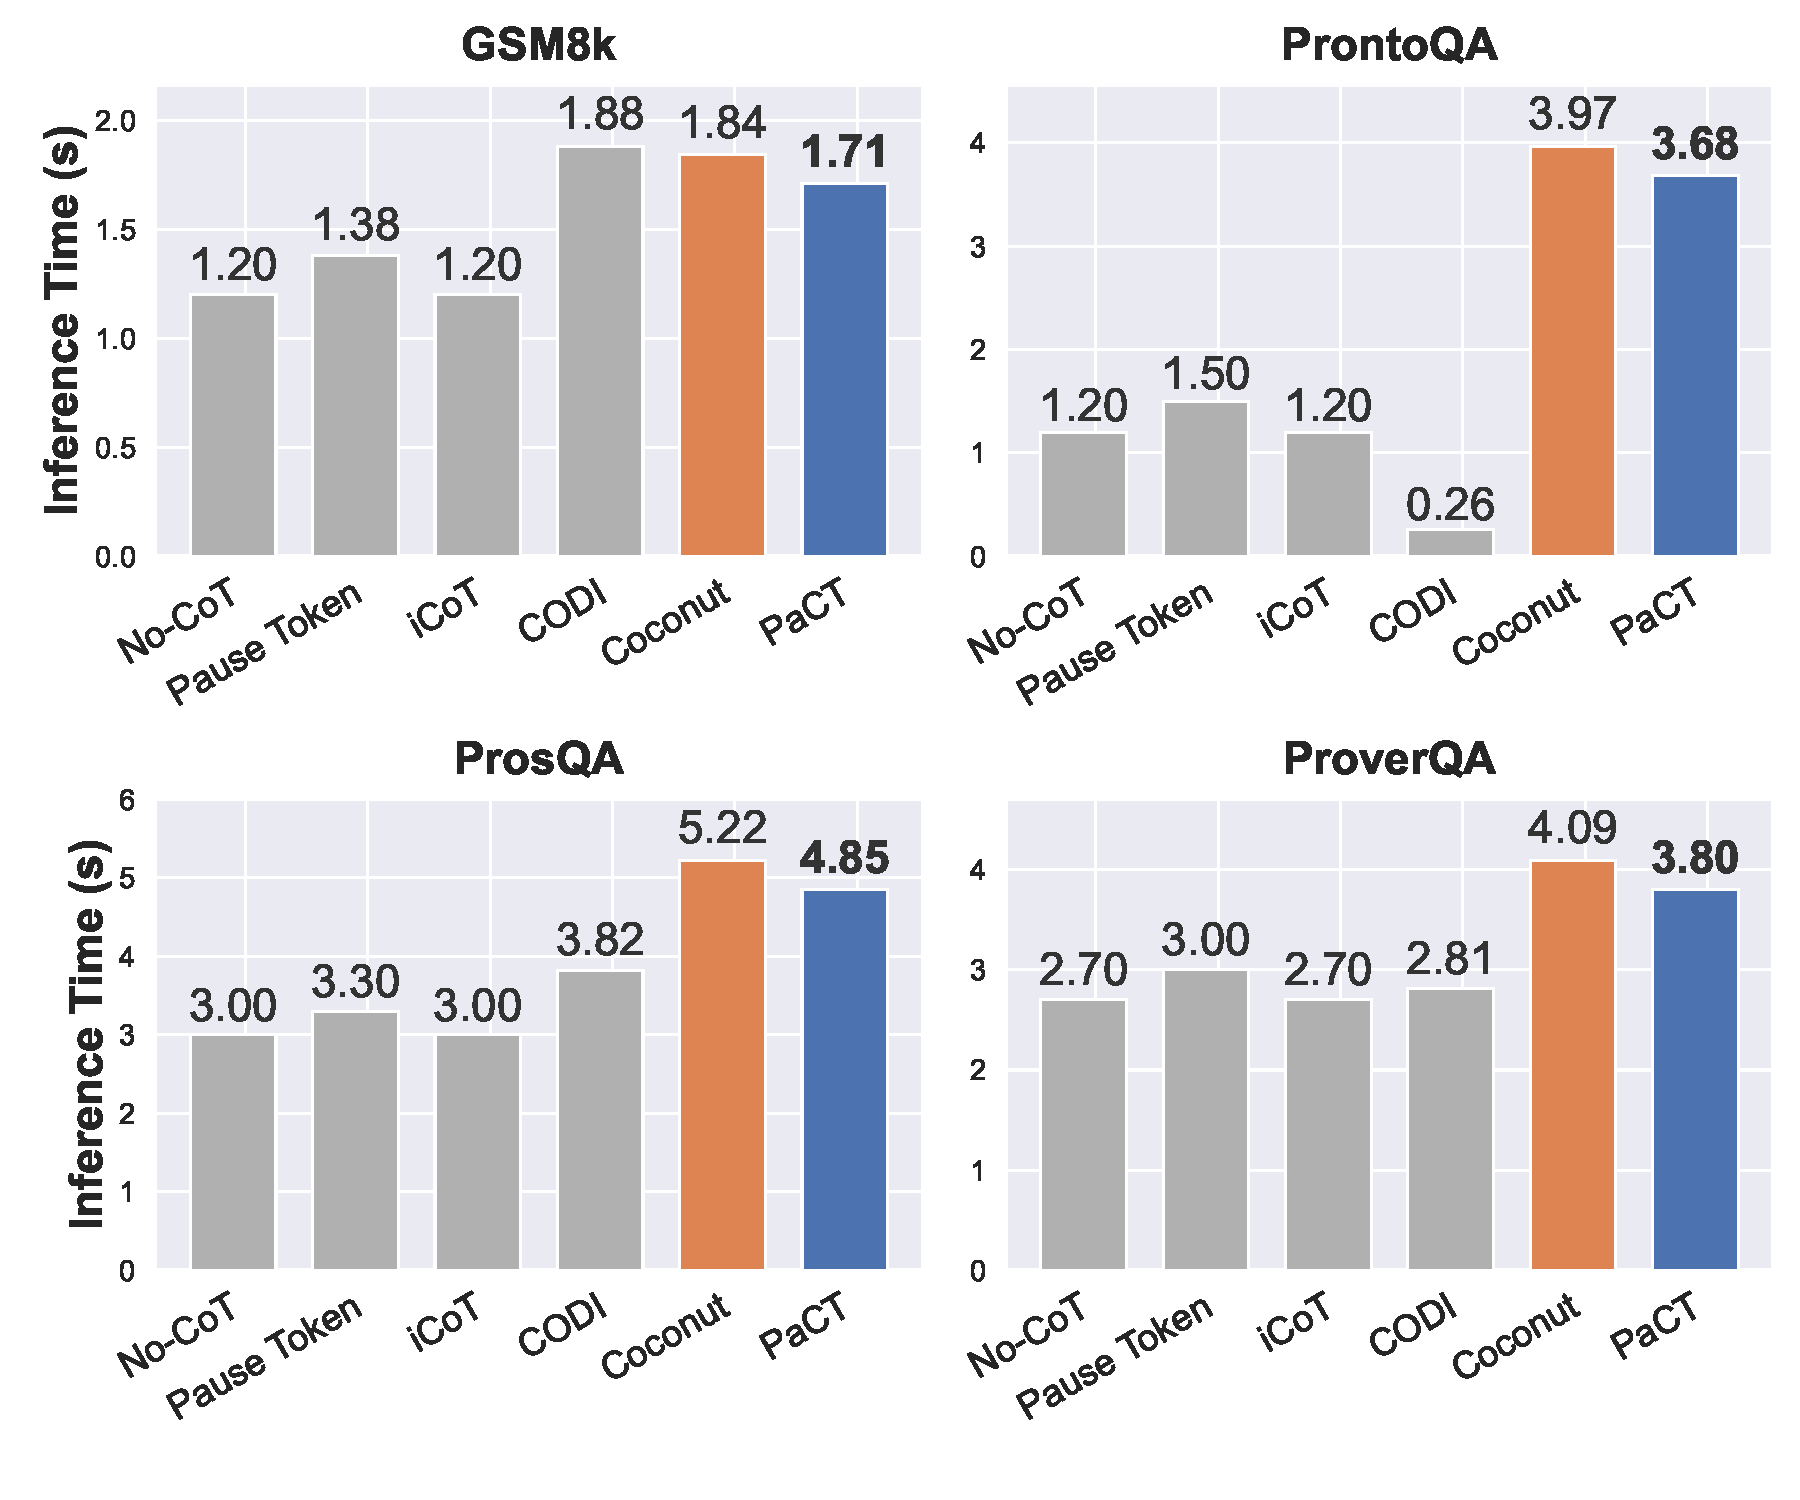
\includegraphics[width=\linewidth]{imgs/inference_times.pdf}
  \caption{\textbf{Inference time (seconds).} Inference time (per sample) for different reasoning methods across four benchmarks.
  PaCT reduces latency relative to Coconut by removing recurrent latent-unrolling overhead, while preserving competitive performance.
  }
  \label{fig:inference_time}
\end{figure}

Figure~\ref{fig:inference_time} reports inference time. PaCT is consistently faster than Coconut, though the
relative gain is smaller than for training because autoregressive answer decoding remains a dominant cost. This is an expected behavior as PaCT primarily removes serial dependence during latent generation; it does not change the causal decoding
interface for answer tokens.

\section{Source Code and Model Availability}
\label{sec:code_release}

To support reproducibility and facilitate future research, we release the full source code and trained model weights for PaCT. The repository includes training scripts, evaluation pipelines, and configuration files required to reproduce all experiments reported in this paper.

Our implementation and pretrained models are publicly available at:
\begin{center}
\href{https://anonymous.4open.science/r/pact-576C/}{\texttt{https://anonymous.4open.science/r/pact-576C/}}
\end{center}




% \subsection{Robustness to perturbations in early latent states}
% \label{sec:latent_robustness}

% Our latent similarity analysis (Table~\ref{tab:latent_similarity}) shows a clear structural difference between PaCT and
% Coconut: PaCT exhibits low cross-stage similarity, indicating stage-wise specialization, while Coconut exhibits high
% cross-stage similarity, suggesting that information is tightly coupled and propagated across latent steps. This motivates
% a robustness test: \emph{if early latent states are perturbed, methods with stronger cross-stage coupling should be more
% sensitive, as errors are carried forward through the latent trajectory.}

% \paragraph{Setup.}
% We evaluate robustness by perturbing only the \emph{first} latent stage at inference time and measuring the resulting
% change in answer accuracy. Let $Z^{(1)} \in \mathbb{R}^{L \times d}$ denote the stage-1 latent states. We consider two
% perturbations: (i) \textbf{additive Gaussian noise}, $\tilde{Z}^{(1)} = Z^{(1)} + \sigma \epsilon$ with
% $\epsilon \sim \mathcal{N}(0, I)$, and (ii) \textbf{magnitude scaling}, $\tilde{Z}^{(1)} = \alpha Z^{(1)}$.
% All subsequent latent stages are computed normally, using the perturbed stage-1 interface.

% \begin{table}[t]
% \centering
% \small
% \caption{\textbf{Robustness to perturbing the first latent stage.} Accuracy (\%) under stage-1 latent perturbations.
% PaCT exhibits smaller degradation than Coconut, consistent with reduced cross-stage coupling.}
% \label{tab:latent_perturbation_robustness}
% \begin{tabular}{lccc}
% \toprule
% Method & Clean & Gaussian ($\sigma{=}0.05$) & Scale ($\alpha{=}0.8$) \\
% \midrule
% Coconut & 32.0 $\pm$ 1.5 & 27.4 $\pm$ 1.7 & 29.8 $\pm$ 1.6 \\
% PaCT    & 34.4 $\pm$ 0.1 & 33.1 $\pm$ 0.2 & 33.6 $\pm$ 0.2 \\
% \bottomrule
% \end{tabular}
% \end{table}

% As shown in Table~\ref{tab:latent_perturbation_robustness}, perturbing the first latent stage leads to a substantially
% larger accuracy drop for Coconut than for PaCT. This aligns with the similarity analysis: Coconut’s higher cross-stage
% similarity indicates that latent states are more tightly coupled, so perturbations introduced early are propagated and
% amplified through recurrent unrolling. In contrast, PaCT’s stage-wise resynthesis yields weaker cross-stage dependence,
% allowing later stages to re-ground latent computation in context and partially correct early perturbations. These results
% provide additional evidence that PaCT’s parallel, non-recurrent latent design improves not only efficiency but also the
% stability of latent reasoning.



% \begin{table}[t]
% \centering
% \begin{tabular}{lcc}
% \toprule
% Method & Peak VRAM (GB) & TFLOPS \\
% \midrule
% Coconut    & 21 &  \\
% CoLaR      & 20 & 11.5 \\
% CODI       & -- &  \\
% \textbf{PaCT} & 28 &  \\
% \bottomrule
% \end{tabular}
% \caption{\textbf{Peak GPU memory usage on a single dataset.}
% Peak VRAM is measured during training for one dataset under a fixed hardware and batch-size configuration.}
% \label{tab:vram_usage}
% \end{table}




\end{document}